% !TeX spellcheck = en_GB
% !TEX program = xelatex+makeindex+bibtex
% !TeX TXS-program:pdflatex = txs:///xelatex %
\documentclass[final,a4paper]{report} %scrreprt of scrartcl
%!TEX program=xelatex+makeindex+bibtex
% Include all project wide packages here.
\usepackage{fullpage}
\usepackage{polyglossia}
\setmainlanguage{english}
\usepackage{csquotes}
\usepackage{graphicx}
\usepackage{epstopdf}
\usepackage{pdfpages}
\usepackage{caption}
\usepackage[list=true]{subcaption}
\usepackage{float}
\usepackage{standalone}
\usepackage{import}
\usepackage{tocloft}
\usepackage{wrapfig}
\usepackage{authblk}
\usepackage{array}
\usepackage{booktabs}
\usepackage[toc,page,title,titletoc]{appendix}
\usepackage{xunicode}
\usepackage{fontspec}
\usepackage{pgfplots}
\usepackage{SIunitx}
\usepackage{units}
\pgfplotsset{compat=newest}
\pgfplotsset{plot coordinates/math parser=false}
\newlength\figureheight 
\newlength\figurewidth
\usepackage{amsmath}
\usepackage{mathtools}
\usepackage{unicode-math}
\usepackage{rotating}
\usepackage{fancyhdr}
\usepackage{titlesec}
\usepackage{blindtext}
\usepackage{color}
\usepackage[margin=3.5cm,headheight=35pt]{geometry}
\usepackage[
    backend=bibtexu,
	texencoding=utf8,
bibencoding=utf8,
    style=ieee,
    sortlocale=en_US,
    language=auto
]{biblatex}
\usepackage{listings}
\usepackage{wrapfig}
\newcommand{\includecode}[4][c]{\lstinputlisting[caption=#2, escapechar=, style=#1,label=#4]{#3}}
\newcommand{\superscript}[1]{\ensuremath{^{\textrm{#1}}}}
\newcommand{\subscript}[1]{\ensuremath{_{\textrm{#1}}}}


\newcommand{\chapternumber}{\thechapter}
\renewcommand{\appendixname}{Appendix}
\renewcommand{\appendixtocname}{Appendices}
\renewcommand{\appendixpagename}{Appendices}

\usepackage[hidelinks]{hyperref} %<--------ALTIJD ALS LAATSTE

%!TEX program=xelatex+makeindex+bibtex
\renewcommand{\familydefault}{\sfdefault}

\setmainfont[Ligatures=TeX]{Calibri}
\setmathfont{Asana Math}
\setmonofont{Lucida Console}

%\definecolor{chapterbarcolor}{cmyk}{.52,.32,0,0}
%\definecolor{footrulecolor}{cmyk}{.52,.32,0,0}

\definecolor{chapterbarcolor}{gray}{0.75}
\definecolor{footrulecolor}{gray}{0.75}

\fancypagestyle{plain}{%
  \fancyhf{}    
  \fancyfoot[L]{\ifnum\value{chapter}>0 \chaptername\ \thechapter. \fi}
  \fancyfoot[C]{\thepage}
  \fancyfoot[R]{\small \today}
  \renewcommand{\headrulewidth}{0pt}
  \renewcommand{\footrulewidth}{2pt}
  \renewcommand{\footrule}{\hbox to\headwidth{%
  \color{footrulecolor}\leaders\hrule height \footrulewidth\hfill}}
}

\pagestyle{plain}

\newcommand{\hsp}{\hspace{20pt}}
\titleformat{\chapter}[hang]{\Huge\bfseries}{\chapternumber\hsp\textcolor{chapterbarcolor}{|}\hsp}{0pt}{\Huge\bfseries}
\titlespacing{\chapter}{0pt}{0pt}{1pt}
\renewcommand{\familydefault}{\sfdefault}
\renewcommand{\arraystretch}{1.2}
\setlength{\headheight}{0pt} 
\setlength\parindent{0pt}
\setlength{\parskip}{0.3cm plus4mm minus3mm}
\setlength\cftaftertoctitleskip{5pt}
\setlength\cftbeforetoctitleskip{20pt}

%For code listings
\definecolor{black}{rgb}{0,0,0}
\definecolor{browntags}{rgb}{0.65,0.1,0.1}
\definecolor{bluestrings}{rgb}{0,0,1}
\definecolor{graycomments}{rgb}{0.4,0.4,0.4}
\definecolor{redkeywords}{rgb}{1,0,0}
\definecolor{bluekeywords}{rgb}{0.13,0.13,0.8}
\definecolor{greencomments}{rgb}{0,0.5,0}
\definecolor{redstrings}{rgb}{0.9,0,0}
\definecolor{purpleidentifiers}{rgb}{0.01,0,0.01}


\lstdefinestyle{csharp}{
language=[Sharp]C,
showspaces=false,
showtabs=false,
breaklines=true,
showstringspaces=false,
breakatwhitespace=true,
escapeinside={(*@}{@*)},
columns=fullflexible,
commentstyle=\color{greencomments},
keywordstyle=\color{bluekeywords}\bfseries,
stringstyle=\color{redstrings},
identifierstyle=\color{purpleidentifiers},
basicstyle=\ttfamily\small}

\lstdefinestyle{c}{
language=C,
showspaces=false,
showtabs=false,
breaklines=true,
showstringspaces=false,
breakatwhitespace=true,
escapeinside={(*@}{@*)},
columns=fullflexible,
commentstyle=\color{greencomments},
keywordstyle=\color{bluekeywords}\bfseries,
stringstyle=\color{redstrings},
identifierstyle=\color{purpleidentifiers},
}

\lstdefinestyle{matlab}{
language=Matlab,
showspaces=false,
showtabs=false,
breaklines=true,
showstringspaces=false,
breakatwhitespace=true,
escapeinside={(*@}{@*)},
columns=fullflexible,
commentstyle=\color{greencomments},
keywordstyle=\color{bluekeywords}\bfseries,
stringstyle=\color{redstrings},
identifierstyle=\color{purpleidentifiers}
}

\lstdefinestyle{vhdl}{
language=VHDL,
showspaces=false,
showtabs=false,
breaklines=true,
showstringspaces=false,
breakatwhitespace=true,
escapeinside={(*@}{@*)},
columns=fullflexible,
commentstyle=\color{greencomments},
keywordstyle=\color{bluekeywords}\bfseries,
stringstyle=\color{redstrings},
identifierstyle=\color{purpleidentifiers}
}

\lstdefinestyle{xaml}{
language=XML,
showspaces=false,
showtabs=false,
breaklines=true,
showstringspaces=false,
breakatwhitespace=true,
escapeinside={(*@}{@*)},
columns=fullflexible,
commentstyle=\color{greencomments},
keywordstyle=\color{redkeywords},
stringstyle=\color{bluestrings},
tagstyle=\color{browntags},
morestring=[b]",
  morecomment=[s]{<?}{?>},
  morekeywords={xmlns,version,typex:AsyncRecords,x:Arguments,x:Boolean,x:Byte,x:Char,x:Class,x:ClassAttributes,x:ClassModifier,x:Code,x:ConnectionId,x:Decimal,x:Double,x:FactoryMethod,x:FieldModifier,x:Int16,x:Int32,x:Int64,x:Key,x:Members,x:Name,x:Object,x:Property,x:Shared,x:Single,x:String,x:Subclass,x:SynchronousMode,x:TimeSpan,x:TypeArguments,x:Uid,x:Uri,x:XData,Grid.Column,Grid.ColumnSpan,Click,ClipToBounds,Content,DropDownOpened,FontSize,Foreground,Header,Height,HorizontalAlignment,HorizontalContentAlignment,IsCancel,IsDefault,IsEnabled,IsSelected,Margin,MinHeight,MinWidth,Padding,SnapsToDevicePixels,Target,TextWrapping,Title,VerticalAlignment,VerticalContentAlignment,Width,WindowStartupLocation,Binding,Mode,OneWay,xmlns:x}
}

%defaults
\lstset{
basicstyle=\ttfamily\scriptsize ,
extendedchars=false,
numbers=left,
numberstyle=\ttfamily\tiny,
stepnumber=1,
tabsize=4,
numbersep=5pt
}
\addbibresource{../../../library/bibliography.bib}
\author{Fairphone Repair Group}
\title{Fairphone Repairability}
\date{\today}
\begin{document}
\section{Hardware}
\label{sec:scrw-it-hardware}
To give the card extra functionality, the decision was made to include the hardware to diagnose the phone into the card.
To make this possible it is necessary to connect the phone to a computer (called a host) through the card. In this section, a description of how this system would work is provided, analysing the host side, the phone's side and finally the card itself with the appropriate components.

\subsection{Host side}
The choice was made to use a standard USB protocol to connect to the host through the card, since the phones uses the same method to connect to the grid to charge or to a computer to communicate.
The USB protocol offers more than enough bandwidth to accomplish the task.
There will also be a little bit of flash memory, for instance \SI{1}{\gibi\bit}, within the card which will be usable like any USB stick and will contain the necessary software to run the diagnostics and for example a script to update the diagnostic software.
The host will issue all the commands that need to be sent to the phone. The only thing the card's hardware does, is translate these to the correct signals on the phone side.
It will act like a transparent proxy who removes the excess USB protocol information from the packages so JTAG communication remains.

\subsection{Phone side}
%TODO Define JTAG, IC
To connect to the phones, a JTAG protocol was selected because nearly all IC's these days have a JTAG protocol interface.
%TODO Define ARM? (really?), SoC
The most important part the ARM based SoC (System-on-a-Chip) used in the phone, has a very well specified JTAG specification.
%TODO Define daisy chain? bus?
The cool thing with JTAG is that you can daisy chain all the different IC's on the same bus.
Originally, JTAG was meant to be a way to test printed circuit board using boundary scan, however nowadays many manufacturers have extended their JTAG implementation to add debug information and for example ROM or flash programming functions.
This tool can even be used instead of a very expensive JTAG debugger in the actual development of the phone.

\subsection{Components}
\begin{table}[h]
	\centering
	\caption{MCU STM32F103R4H6A}
	\label{tab:mcu-specs}		
	\begin{tabular}{ll}
		\toprule		
		Key & Value \\
		\hline
		Architecture & ARM Cortex-M3 \\
		Max Clock & \SI{72}{\mega\hertz} \\
		Package & TFBGA \\
		No. of Pins & 64 \\
		No of IOs & 51 \\
		Flash & \SI{16}{\kibi\byte} \\
		RAM & \SI{6}{\kibi\byte} \\
		Supply Voltage Max & \SI{3.6}{\volt} \\
		Supply Voltage Min & \SI{2.0}{\volt} \\
		\bottomrule
	\end{tabular}
\end{table}

\begin{table}[h]
	\centering
	\caption{Flash S34ML01G200BHI000}
	\label{tab:flash-specs}
	\begin{tabular}{ll}
		\toprule		
		Key & Value \\
		\hline
		Access time & \SI{25}{\nano\second} \\
		Flash Configuration & 128\si{\mebi} x \SI{8}{\bit} \\
		Package & BGA \\
		No. of Pins & 63 \\
		Size & Flash - NAND \\	
		Interface & Parallel \\
		Size & \SI{1}{\gibi\bit} \\		
		Supply Voltage Max & \SI{3.6}{\volt} \\
		Supply Voltage Min & \SI{2.7}{\volt} \\
		\bottomrule
	\end{tabular}
\end{table}

\begin{table}[h]
	\centering
	\caption{micro-USB B pinout}
	\label{tab:microusb-pinout}		
	\begin{tabular}{lllp{6cm}}
		\toprule		
		Pin & Name & Cable color & Description\\
		\hline
		1 & VCC & Red & +5 VDC\\
		2 & D- & White & Data -\\
		3 & D+ & Green & Data +\\
		4 & ID &  & Mode Detect. May be N/C, GND or used as an attached device presence indicator (shorted to GND with resistor)\\
		5 & GND & Black & Ground\\
		\bottomrule
	\end{tabular}
\end{table}

First we need the ``brain'' of the hardware.
We chose a 32-bit ARM Cortex-M3 based MCU made by STMICROELECTRONICS.
This MCU has a USB interface built-in and it has 51 IO pins.
Other specifications are shown in Table \ref{tab:mcu-specs}.
Second we need the appropriate receptacle to put the micro USB cable in.
We chose one that is reclined one and of type B so the overall thickness on the hardware stays down.
It needs to fit in the card without making the card to thick of the walls too thin.

We need two pins on the MCU for the USB interface, the other three pins are ID, GND and VCC (\SI{5}{\volt}).
Pinout in Table \ref{tab:microusb-pinout}.
%TODO cite datasheet MCU page 69
We need to add a \SI{1.5}{\kilo\ohm} pull-up resistor to the D+ pin to pull it up to the \SIrange{3.0}{3.6}{\volt} range so we are USB2.0 compliant.
We also want to add flash memory to ship the required software, we chose a \SI{1}{\gibi\bit} chip with a parallel interface.
We will need 15 to 16 pins on the MCU for the flash depending on the configuration.
Specifications are in Table \ref{tab:flash-specs}
To connect to the phone we will need the JTAG 20 pin connector, we chose a 1mm pinch connector.

To support all this we need to convert the \SI{5}{\volt} VCC voltage to a workable \SI{3.3}{\volt} for use with all the ARM based chips, the flash and the phone.
We will also add a power filter, crystal oscillator, supporting flash circuits and supporting ARM circuits.
The supporting circuits are to make sure that the chips boot correctly without damaging themselves.
This also protects the circuit against electronic static discharge and sudden power loss.
%TODO connector pictures
\begin{figure}[H]
	\centering
	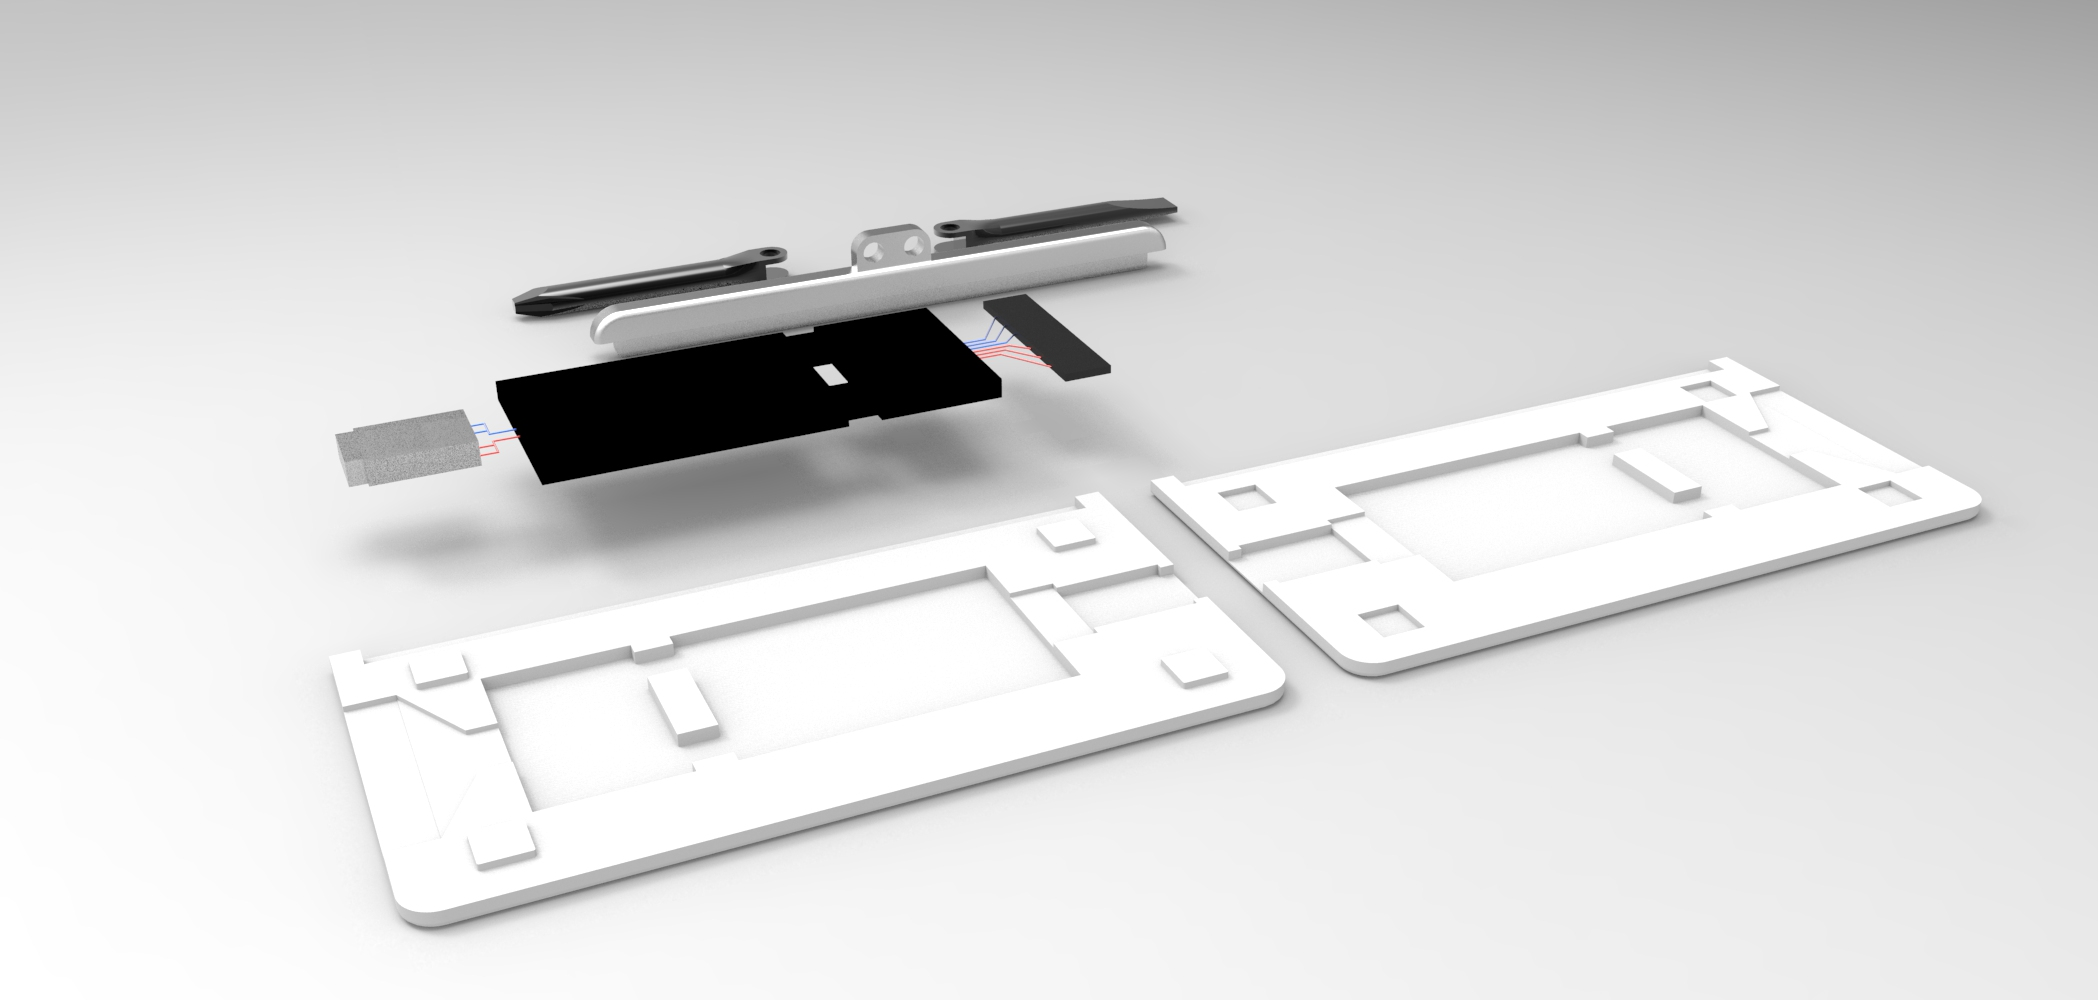
\includegraphics[width=0.8\textwidth]{resources/CardDesign3}
	\caption{Card interior hardware design}
	\label{fig:CardInteriorHardwareDesign}
\end{figure}
\end{document}
